\documentclass[submit]{harvardml}

\course{CS181-S22}
\assignment{Assignment \#6}
\duedate{11:59PM EST, April 29 2022}
\newcommand{\attr}[1]{\textsf{#1}}
\usepackage[OT1]{fontenc}
\usepackage{float}
\usepackage[colorlinks,citecolor=blue,urlcolor=blue]{hyperref}
\usepackage[pdftex]{graphicx}
\usepackage{subfig}
\usepackage{fullpage}
\usepackage{amsmath}
\usepackage{amssymb}
\usepackage{color}
\usepackage{todonotes}
\usepackage{listings}
\usepackage{common}
\usepackage{bm}
\usepackage{enumitem}
\usepackage{tikz}
\usepackage{xifthen}
\usepackage{soul}
\usepackage{framed}
\usepackage{xcolor}
\newcommand{\mathcolorbox}[2]{\colorbox{#1}{$\displaystyle #2$}}

\usepackage[mmddyyyy,hhmmss]{datetime}

\definecolor{verbgray}{gray}{0.9}

\lstnewenvironment{csv}{
  \lstset{backgroundcolor=\color{verbgray},
  frame=single,
  framerule=0pt,
  basicstyle=\ttfamily,
  columns=fullflexible}}{}

\newcommand{\mueps}{\mu_{\epsilon}}
\newcommand{\sigeps}{\sigma_{\epsilon}}
\newcommand{\mugam}{\mu_{\gamma}}
\newcommand{\siggam}{\sigma_{\gamma}}
\newcommand{\muzp}{\mu_{p}}
\newcommand{\sigzp}{\sigma_{p}}
\newcommand{\gauss}[3]{\frac{1}{2\pi#3}e^{-\frac{(#1-#2)^2}{2#3}}}


\begin{document}
\begin{center}
{\Large Homework 6: Inference in Graphical Models, MDPs}\\
\end{center}

\subsection*{Introduction}

In this assignment, you will practice inference in graphical models as
well as MDPs/RL.  For readings, we recommend \href{http://incompleteideas.net/book/the-book-2nd.html}{Sutton and Barto 2018, Reinforcement Learning: An Introduction}, \href{https://harvard-ml-courses.github.io/cs181-web-2017/}{CS181 2017 Lecture Notes}, and Section 10 and 11 Notes.

Please type your solutions after the corresponding problems using this
\LaTeX\ template, and start each problem on a new page.

Please submit the \textbf{writeup PDF to the Gradescope assignment `HW6'}. Remember to assign pages for each question.

Please submit your \textbf{\LaTeX\ file and code files to the Gradescope assignment `HW6 - Supplemental'}. 

You can use a \textbf{maximum of 2 late days} on this assignment.  Late days will be counted based on the latest of your submissions. 
\\

\newpage

\begin{problem}[Explaining Away + Variable Elimination 15 pts]

  In this problem, you will carefully work out a basic example with
  the ``explaining away'' effect. There are many derivations of this
  problem available in textbooks. We emphasize that while you may
  refer to textbooks and other online resources for understanding how
  to do the computation, you should do the computation below from
  scratch, by hand.

  We have three binary variables: rain $R$, wet grass $G$, and
  sprinkler $S$.
We  assume the following factorization of the joint distribution:
$$
\Pr(R,S,G) = \Pr(R)\Pr(S)\Pr(G\, |\, R, S).
  $$
  
  The conditional probability tables look like the
  following:
  \begin{eqnarray*}
    \Pr(R = 1) &= 0.25 \\
    \Pr(S = 1) &= 0.5 \\
    \Pr(G = 1 | R = 0 , S = 0 ) &= 0 \\
    \Pr(G = 1 | R = 1 , S = 0 ) &= .75 \\
    \Pr(G = 1 | R = 0 , S = 1 ) &= .75 \\
    \Pr(G = 1 | R = 1 , S = 1 ) &= 1
  \end{eqnarray*}
  
 
  \begin{enumerate}
    \item Draw the graphical model corresponding to the
      factorization. Are $R$ and $S$ independent?  [Feel free to use
      facts you have learned about studying independence in graphical models.]
    \item You notice it is raining and check on the sprinkler without
      checking the grass.  What is the probability that it is on?
    \item You notice that the grass is wet and go to check on the
      sprinkler (without checking if it is raining).  What is the
      probability that it is on?
    \item You notice that it is raining and the grass is wet.  You go
      check on the sprinkler.  What is the probability that it is on?
    \item What is the ``explaining away'' effect that is shown above?
    \end{enumerate}
    
Consider if we introduce a new binary variable, cloudy $C$, to the the original three binary variables such that the factorization of the joint distribution is now: 

$$
\Pr(C, R,S,G) = \Pr(C)\Pr(R|C)\Pr(S|C)\Pr(G\, |\, R, S).
$$

\begin{enumerate}
    \setcounter{enumi}{5}
    \item For the marginal distribution $\Pr(R)$, write down the variable elimination expression with the elimination ordering $S, G, C$ (where $S$ is eliminated first, then $G$, then $C$).
    \item For the marginal distribution $\Pr(R)$, write down the variable elimination expression with the elimination ordering $C,G,S$.
    \item Give the complexities for each ordering. Which elimination ordering takes less computation?
\end{enumerate}
\end{problem}
\newpage

\textbf{Solution:}\\
\textbf{Solution 1:}
\begin{center}
\begin{tikzpicture}[
  node distance=1cm and .5cm,
  bn/.style={draw,circle,text width=2cm,align=center}
    ]
    \node[bn] (w) {\attr{G}};
    \node[bn,above right=of w] (t) {\attr{S}};
    \node[bn,above left=of w] (f) {\attr{R}};
    \path (t) edge[-latex] (w)
    (f) edge[-latex] (w);
    \end{tikzpicture}
\end{center}

\textbf{Solution 2:}\\
S and R are d-separated by G when G is not observed, i.e. S and R are independent conditional upon not observing G. Therefore, the probability that the sprinkler is on given it is raining (without checking the grass) is given by:
\begin{align*}
     \Pr(S = 1 | R = 1) &= \Pr(S = 1)\\
     &= \mathcolorbox{green}{0.5}
\end{align*}

\textbf{Solution 3:}\\
Using Bayes' rule, the probability that the sprinkler is on given the grass is wet (without checking that it is raining) is given by:
\begin{align*}
     \Pr(S = 1 | G = 1) &= \frac{\Pr(G = 1 | S = 1) \Pr(S=1)}{\Pr(G=1)}
\end{align*}
We can calculate the components of this expression individually.\\

Using the law of total probability by conditioning on the possible states of $R$ and $S$ and noting (from 2) that $R$ and $S$ are d-separated, when $G$ is not observed:
\begin{align*}
    \Pr(G=1) &= \Pr(G=1|R=1,S=1)\Pr(R=1)\Pr(S=1)\\ &\quad+ \Pr(G=1|R=0,S=1)\Pr(R=0)\Pr(S=1)\\ &\quad+ \Pr(G=1|R=1,S=0)\Pr(R=1)\Pr(S=0)\\ &\quad+ \Pr(G=1|R=0,S=0)\Pr(R=0)\Pr(S=0)\\
    &= 1(0.25)(0.5) + (0.75)(0.75)(0.5) + (0.75)(0.25)(0.5) + 0\\
    &= 0.5
\end{align*}
Using the law of total probability by conditioning on the possible states of $R$:
\begin{align*}
    \Pr(G=1|S=1) &= \Pr(G=1|S=1,R=1)\Pr(R=1)\\ &\quad+ \Pr(G=1|S=1,R=0)\Pr(R=0)\\
    &= 1(0.25) + (0.75)(0.75)\\
    &= \frac{13}{16}
\end{align*}
And, using what is already given:
\begin{align*}
    \Pr(S=1) = 0.5
\end{align*}
Putting this all together, we get that:
\begin{align*}
     \Pr(S = 1 | G = 1) &= \frac{\frac{13}{16}\cdot(0.5)}{0.5} = \frac{13}{16} = \mathcolorbox{green}{0.8125}
\end{align*}

\textbf{Solution 4:}\\
Using simple rules of conditional probability, the probability that the sprinkler is on given the grass is wet and given that it is raining is:
\begin{align*}
     \Pr(S = 1 | R = 1, G = 1) &= \frac{\Pr(G = 1, R = 1, S = 1)}{\Pr(R=1,G=1)}\\
     &= \frac{\Pr(G = 1| R = 1, S = 1)\Pr(R=1)\Pr(S=1)}{\Pr(R=1,G=1,S=1) + \Pr(R=1,G=1, S=0)}\\
     &= \frac{\Pr(G = 1| R = 1, S = 1)\Pr(R=1)\Pr(S=1)}{\Pr(R=1)\Pr(S=1)\Pr(G=1|R=1,S=1) + \Pr(R=1)\Pr(S=0)\Pr(G=1|R=1,S=0)}
\end{align*}
which has been simplified using the law of total probability in the denominator by conditioning on the possible states of $S$ and noting (from 2) that $R$ and $S$ are d-separated, when $G$ is not observed.

\begin{align*}
     \therefore \Pr(S = 1 | R = 1, G = 1) &= \frac{(0.25)(0.5)(1)}{(0.25)(0.5)(1)+(0.25)(0.5)(0.75)}\\
     &= \frac{4}{7} \approx \mathcolorbox{green}{0.571}
\end{align*}

\textbf{Solution 5:}\\
Noticing that the probability calculated in 4 is lower than the probability calculated in 3, we can conclude that observing there being rain ``explains away" the effect of the sprinkler on the grass. In other words, having observed that the grass is wet and that it is raining, it makes it less likely that the grass was made wet by the sprinkler too, than had we just observed the grass being wet.\\

Note, that this explaining away effect at $G$ only occurs because we observe $G$ in both cases, thereby unblocking the path between $R$ and $S$, meaning they are no longer independent, so knowing either of $R$ or $S$ changes the amount we expected the other of $R$ or $S$ to contribute to $G$ - exactly the ``explaining away" effect.
\newpage

\textbf{Solution 6:}\\
\begin{align*}
    \Pr(R) &= \sum_C \sum_G \sum_S \Pr(C,R,G,S)\\
    &= \sum_C \sum_G \sum_S \Pr(C)\Pr(R|C)\Pr(S|C)\Pr(G | R, S)\\
    &= \mathcolorbox{green}{\sum_C \Pr(C)\Pr(R|C) \sum_G \sum_S \Pr(S|C)\Pr(G | R, S)}\\
    &= \sum_C \Pr(C)\Pr(R|C) \sum_G \sum_S \psi_1(G,C,R,S)\\
    &= \sum_C \Pr(C)\Pr(R|C) \sum_G \psi_2(G,C,R)\\
    &= \sum_C \psi_3(C,R)\\
    &= \Pr(R)
\end{align*}

\textbf{Solution 7:}\\
\begin{align*}
    \Pr(R) &= \sum_S \sum_G \sum_C \Pr(C,R,G,S)\\
    &= \sum_S \sum_G \sum_C \Pr(C)\Pr(R|C)\Pr(S|C)\Pr(G | R, S)\\
    &= \mathcolorbox{green}{\sum_S \sum_G \Pr(G | R, S) \sum_C \Pr(C)\Pr(R|C)\Pr(S|C)}\\
    &= \sum_S \sum_G \Pr(G | R, S) \sum_C \psi_1(C,R,S)\\
    &= \sum_S \sum_G \psi_2(G,R,S)\\
    &= \sum_S \psi_3(R,S)\\
    &= \Pr(R)
\end{align*}

\textbf{Solution 8:}\\
In question 6, we see that the variable elimination involves summing over a $k^4$ sized object $\psi_1(G,C,R,S)$, followed by a $k^3$ sized object $\psi_2(G,C,R)$, followed by a $k^2$ sized object $\psi_3(C,R)$. Therefore, the variable elimination ordering $S,G,C$ has time complexity:
$$O(k^4)+O(k^3)+O(k^2) = \mathcolorbox{green}{O(k^4)}$$

In question 7, we see that the variable elimination involves summing over a $k^3$ sized object $\psi_1(C,R,S)$, followed by a $k^3$ sized object $\psi_2(G,R,S)$, followed by a $k^2$ sized object $\psi_3(R,S)$. Therefore, the variable elimination ordering $C,G,S$ has time complexity:
$$O(k^3)+O(k^3)+O(k^2) = \mathcolorbox{green}{O(k^3)}$$

Therefore, the variable elimination ordering $C,G,S$ takes less computation.

\newpage


\begin{problem}[Policy and Value Iteration, 15 pts]

This question asks you to implement policy and value iteration in a
simple environment called Gridworld.  The ``states'' in Gridworld are
represented by locations in a two-dimensional space.  Here we show each state and its reward:

\begin{center}
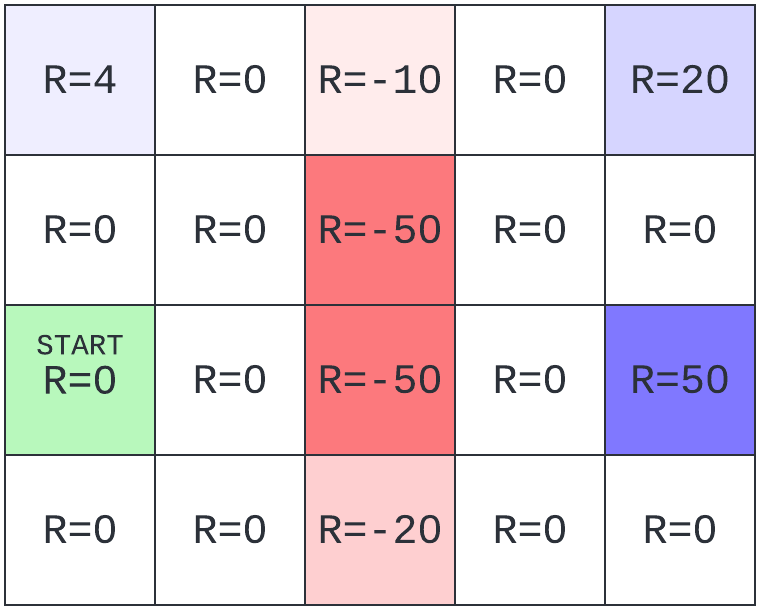
\includegraphics[width=3in]{gridworld.png}
\end{center}
The set of actions is \{N, S, E, W\}, which corresponds to moving north (up), south (down), east (right), and west (left) on the grid.
Taking an action in Gridworld does not always succeed with probability
$1$; instead the agent has probability $0.1$ of ``slipping'' into a
state on either side, but not backwards.  For example, if the agent tries to move right from START, it succeeds with probability 0.8, but the agent may end up moving up or down with probability 0.1 each. Also, the agent cannot move off the edge of the grid, so moving left from START will keep the agent in the same state with probability 0.8, but also may slip up or down with probability 0.1 each. Lastly, the agent has no chance of slipping off the grid - so moving up from START results in a 0.9 chance of success with a 0.1 chance of moving right.

Your job is to implement the following three methods in file \texttt{T6\_P2.ipynb}. Please use the provided helper functions \texttt{get\_reward} and \texttt{get\_transition\_prob} to implement your solution.

\emph{Do not use any outside code.  (You may still collaborate with others according to the standard collaboration policy in the syllabus.)}  

\emph{Embed all plots in your writeup.}
\end{problem}
\newpage

\begin{framed}
\textbf{Problem 2} (cont.)\\

\textbf{Important: } The state space is represented using integers, which range from 0 (the top left) to 19 (the bottom right). Therefore both the policy \texttt{pi} and the value function \texttt{V} are 1-dimensional arrays of length \texttt{num\_states = 20}. Your policy and value iteration methods should only implement one update step of the iteration - they will be repeatedly called by the provided \texttt{learn\_strategy} method to learn and display the optimal policy. You can change the number of iterations that your code is run and displayed by changing the $\texttt{max\_iter}$ and $\texttt{print\_every}$ parameters of the $\texttt{learn\_strategy}$ function calls at the end of the code.

Note that we are doing infinite-horizon planning to maximize the expected reward of the traveling agent. For parts 1-3, set discount factor $\gamma = 0.7$.

\begin{itemize}
    \item[1a.]  Implement function \texttt{policy\_evaluation}.  Your
      solution should learn value function $V$, either using a closed-form expression or iteratively using
      convergence tolerance $\texttt{theta = 0.0001}$ (i.e., if
      $V^{(t)}$ represents $V$ on the $t$-th iteration of your policy
      evaluation procedure, then if $|V^{(t + 1)}[s] - V^{(t)}[s]|
      \leq \theta$ for all $s$, then terminate and return $V^{(t + 1)}$.)

    \item[1b.] Implement function \texttt{update\_policy\_iteration} to update the policy \texttt{pi} given a value function \texttt{V} using \textbf{one step} of policy iteration.
    
    \item[1c.] Set \texttt{max\_iter = 4}, \texttt{print\_every = 1} to show the learned value function and the associated policy for the first 4 policy iterations. Do not modify the plotting code. Please fit all 4 plots onto one page of your writeup.
    
    \item [1d.] Set \texttt{ct = 0.01} and increase \texttt{max\_iter} such that the algorithm converges. Include a plot of the final learned value function and policy. How many iterations does it take to converge? Now try \texttt{ct = 0.001} and \texttt{ct = 0.0001}. How does this affect the number of iterations until convergence?
      
    \item [2a.] Implement function
      \texttt{update\_value\_iteration}, which performs \textbf{one step} of value iteration to update \texttt{V}, \texttt{pi}.
      
    \item [2b.] Set \texttt{max\_iter = 4}, \texttt{print\_every = 1} to show the learned value function and the associated policy for the first 4 value iterations. Do not modify the plotting code. Please fit all 4 plots onto one page of your writeup.
    
    \item [2c.] Set \texttt{ct = 0.01} and increase \texttt{max\_iter} such that the algorithm converges. Include a plot of the final learned value function and policy. How many iterations does it take to converge? Now try \texttt{ct = 0.001} and \texttt{ct = 0.0001}. How does this affect the number of iterations until convergence?
    
    \item[3] Compare and contrast the number of iterations, time per iteration, and overall runtime between policy iteration and value iteration. What do you notice?
    
    \item[4] Plot the learned policy with each of $\gamma \in (0.6,0.7,0.8,0.9)$. Include all 4 plots in your writeup. Describe what you see and provide explanations for the differences in the observed policies. Also discuss the effect of gamma on the runtime for both policy and value iteration.
    
    \item[5] Now suppose that the game ends at any state with a positive reward, i.e. it immediately transitions you to a new state with zero reward that you cannot transition away from. What do you expect the optimal policy to look like, as a function of gamma? Numerical answers are not required, intuition is sufficient.
 
\end{itemize}
\end{framed}

\newpage
\textbf{Solution:}\\
\textbf{Solution 1(c)}:\\
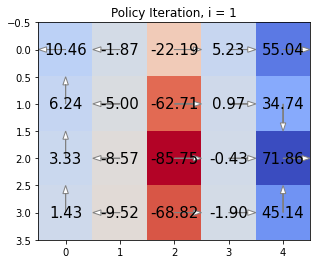
\includegraphics[width=0.5\linewidth]{HW6/plots/1c.1.png}
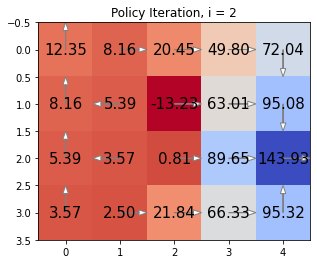
\includegraphics[width=0.5\linewidth]{HW6/plots/1c.2.png}
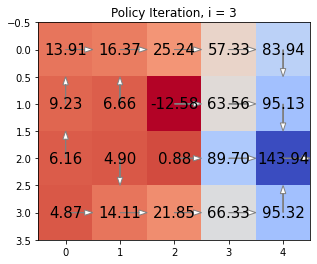
\includegraphics[width=0.5\linewidth]{HW6/plots/1c.3.png}
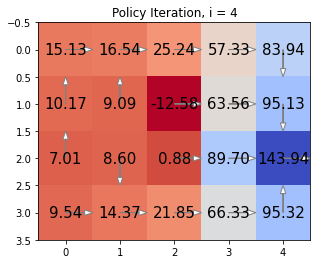
\includegraphics[width=0.5\linewidth]{HW6/plots/1c.4.png}
\newpage

\textbf{Solution 1(d)}:\\
\begin{center}
    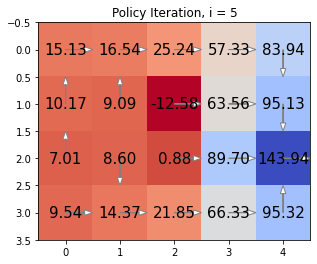
\includegraphics[width=0.5\linewidth]{HW6/plots/1d.ct=0.01.png}
\end{center}
The policy evaluation/iteration algorithm takes 5 iterations to converge. Changing the value of \texttt{ct} does not change the number of iterations until convergence, i.e. it remains at 5. This is intuitive because policy evaluation/iteration should converge to the optimal policy exactly when it converges. 
\newpage

\textbf{Solution 2(b)}:\\
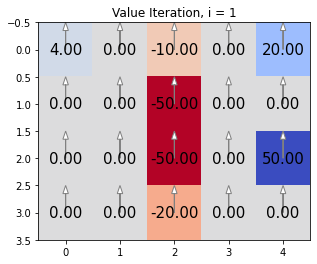
\includegraphics[width=0.5\linewidth]{HW6/plots/2b.1.png}
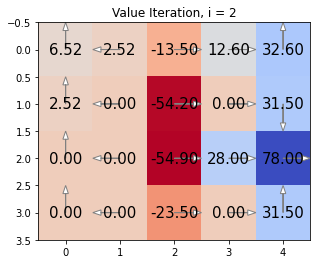
\includegraphics[width=0.5\linewidth]{HW6/plots/2b.2.png}
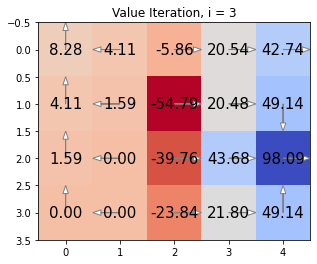
\includegraphics[width=0.5\linewidth]{HW6/plots/2b.3.png}
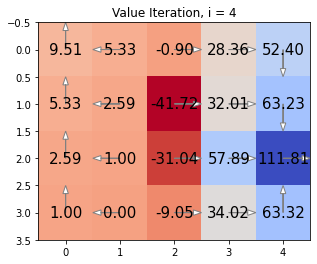
\includegraphics[width=0.5\linewidth]{HW6/plots/2b.4.png}
\newpage

\textbf{Solution 2(c)}:\\
\begin{center}
    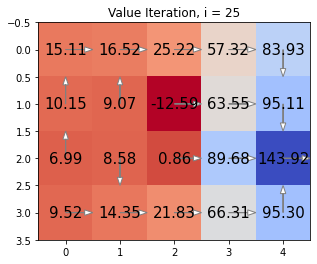
\includegraphics[width=0.5\linewidth]{HW6/plots/2c.ct=0.01.png}
\end{center}
\begin{center}
        \begin{tabular}{ |c|c| } 
        \hline
        \texttt{ct} & Number of iterations until convergence \\
        \hline
        0.01 & 25\\
        \hline
        0.001 & 31\\
        \hline
        0.0001 & 38\\
        \hline
        \end{tabular}
\end{center}
Decreasing the value of \texttt{ct} increases the number of iterations until convergence. This is intuitive because value iteration does not converge exactly, so decreasing the convergence threshold makes it more difficult to achieve the level of accuracy required to converge, and requires more iterations.\\

\textbf{Solution 3}:\\
Using a convergence tolerance of $0.01$:
\begin{center}
        \begin{tabular}{ |c|c|c| } 
        \hline
        & Policy iteration & Value iteration \\
        \hline
        Number of iterations & 5 & 25\\
        \hline
        Time per iteration & 0.682 & 0.260\\
        \hline
        Overall runtime & 3.41 & 6.49\\
        \hline
        \end{tabular}
\end{center}
Policy iteration takes less iterations to converge and takes less time per iteration but takes more time overall to run, when compared to value iteration. This is intuitive, since policy iteration has runtime of $O(|S||A|L + |S|^3)$ per step, and value iteration has runtime of $O(|S||A|L)$ per step, where $|S|$ is defined as the number of states in the world, $|A|$ is defined as the number of possible actions, and $L$ is defined as the maximum number of states reachable from any states through any action. However, policy iteration converges faster overall as it converges exactly and does not need to spend time, unlike value iteration, improving the accuracy of the value function up to the second decimal place, until it reaches the convergence threshold. Thus, value iteration ends up taking many more, albeit shorter iterations, which end up taking longer overall than policy iteration's few, slower iterations.
\newpage

\textbf{Solution 4}:\\
Using a convergence tolerance of $0.01$:
\begin{figure}[h]
    \centering
    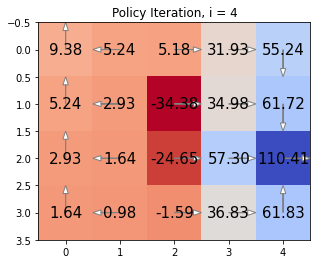
\includegraphics[width=0.5\linewidth]{HW6/plots/2.4.g=0.6.png}
    \caption{\texttt{$\gamma$ = 0.6}}
\end{figure}
\begin{figure}[h]
    \centering
    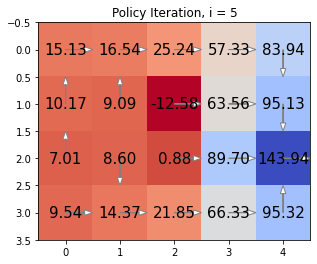
\includegraphics[width=0.5\linewidth]{HW6/plots/2.4.g=0.7.png}
    \caption{\texttt{$\gamma$ = 0.7}}
\end{figure}
\newpage
\begin{figure}[h]
    \centering
    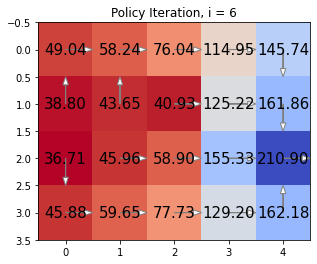
\includegraphics[width=0.5\linewidth]{HW6/plots/2.4.g=0.8.png}
    \caption{\texttt{$\gamma$ = 0.8}}
\end{figure}
\begin{figure}[h]
    \centering
    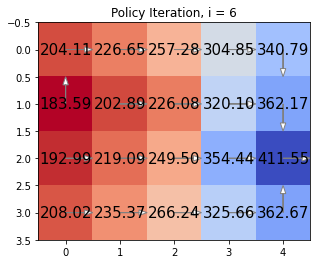
\includegraphics[width=0.5\linewidth]{HW6/plots/2.4.g=0.9.png}
    \caption{\texttt{$\gamma$ = 0.9}}
\end{figure}

\begin{center}
        \begin{tabular}{ |c|c|c| } 
        \hline
        \texttt{$\gamma$} & Policy iteration runtime & Value iteration runtime \\
        \hline
        0.6 & 2.27 & 4.78\\
        \hline
        0.7 & 3.41 & 6.49\\
        \hline
        0.8 & 6.24 & 10.4\\
        \hline
        0.9 & 9.73 & 21.6\\
        \hline
        \end{tabular}
\end{center}
Increasing the magnitude of $\gamma$ decreases the amount of discounting on rewards from future states. Thus, it makes sense for policies to travel further in order to collect more rewards in the future, and the agent travels for more time. This is the case for both value and policy iteration, so the overall runtime increases for both algorithms as $\gamma$ increases.\\

\textbf{Solution 5}:\\
Larger values of $\gamma$ increase the value of future rewards as the level of discounting decreases. Thus, as $\gamma$ tends towards 1, policies will recommend longer paths, as it becomes worthwhile travelling the long path from the start to the grid-square with the highest reward (R=50). Meanwhile, lower values of $\gamma$ decrease the value of future rewards as the level of discounting increases. Thus, policies will take shorter paths, given lower values of $\gamma$, e.g. to the grid-square with R=4, as it is not worth travelling further to only get the heavily discounted R=50 in the future.

\begin{problem}[Reinforcement Learning, 20 pts]
  In 2013, the mobile game \emph{Flappy Bird} took the world by storm. You'll be developing a Q-learning agent to play a similar game, \emph{Swingy Monkey} (See Figure~\ref{fig:swingy}).  In this game, you control a monkey that is trying to swing on vines and avoid tree trunks.  You can either make him jump to a new vine, or have him swing down on the vine he's currently holding.  You get points for successfully passing tree trunks without hitting them, falling off the bottom of the screen, or jumping off the top.  There are some sources of randomness: the monkey's jumps are sometimes higher than others, the gaps in the trees vary vertically, the gravity varies from game to game, and the distances between the trees are different.  You can play the game directly by pushing a key on the keyboard to make the monkey jump.  However, your objective is to build an agent that \emph{learns} to play on its own. 
  
   You will need to install the \verb|pygame| module
  (\url{http://www.pygame.org/wiki/GettingStarted}).
  

\textbf{Task:}
Your task is to use Q-learning to find a policy for the monkey that can navigate the trees.  The implementation of the game itself is in file \verb|SwingyMonkey.py|, along with a few files in the \verb|res/| directory.  A file called \verb|stub.py| is the starter code for setting up your learner that interacts with the game.  This is the only file you need to modify (but to speed up testing, you can comment out the animation rendering code in \verb|SwingyMonkey.py|). You can watch a YouTube video of the staff Q-Learner playing the game at \url{http://youtu.be/l4QjPr1uCac}.  It figures out a reasonable policy in a few dozen iterations.
You'll be responsible for implementing the Python function  \verb|action_callback|. The action callback will take in a dictionary that describes the current state of the game and return an action for the next time step.  This will be a binary action, where 0 means to swing downward and 1 means to jump up.  The dictionary you get for the state looks like this:
\begin{csv}
{ 'score': <current score>,
  'tree': { 'dist': <pixels to next tree trunk>,
            'top':  <height of top of tree trunk gap>,
            'bot':  <height of bottom of tree trunk gap> },
  'monkey': { 'vel': <current monkey y-axis speed>,
              'top': <height of top of monkey>,
              'bot': <height of bottom of monkey> }}
\end{csv}
All of the units here (except score) will be in screen pixels. Figure~\ref{fig:swingy-ann} shows these graphically. 
Note that since the state space is very large (effectively continuous), the monkey's relative position needs to be discretized into bins. The pre-defined function \verb|discretize_state| does this for you.

\textbf{Requirements}
\\
\textit{Code}: First, you should implement Q-learning with an
$\epsilon$-greedy policy yourself. You can increase the performance by
trying out different parameters for the learning rate $\alpha$,
discount rate $\gamma$, and exploration rate $\epsilon$. \emph{Do not use outside RL code for this assignment.} Second, you should use a method of your choice to further improve the performance. This could be inferring gravity at each epoch (the gravity varies from game to game), updating the reward function, trying decaying epsilon greedy functions, changing the features in the state space, and more. One of our staff solutions got scores over 800 before the 100th epoch, but you are only expected to reach scores over 50 before the 100th epoch. {\bf Make sure to turn in your code!} \\\\
\textit{Evaluation}: In 1-2 paragraphs, explain how your agent performed and what decisions you made and why. Make sure to provide evidence where necessary to explain your decisions. You must include in your write up at least one plot or table that details the performances of parameters tried (i.e. plots of score vs. epoch number for different parameters).
\\\\
\textit{Note}: Note that you can simply discretize the state and action spaces and run the Q-learning algorithm. There is no need to use complex models such as neural networks to solve this problem, but you may do so as a fun exercise.

\end{problem}
\begin{figure}[H]
    \centering%
    \subfloat[SwingyMonkey Screenshot]{%
        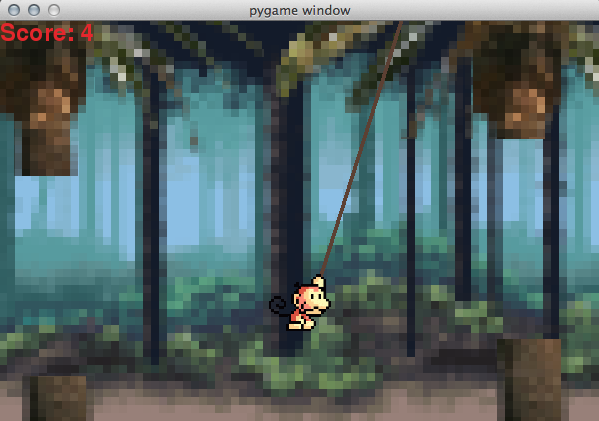
\includegraphics[width=0.48\textwidth]{figures/swingy}
        \label{fig:swingy}
    }\hfill
    \subfloat[SwingyMonkey State]{%
        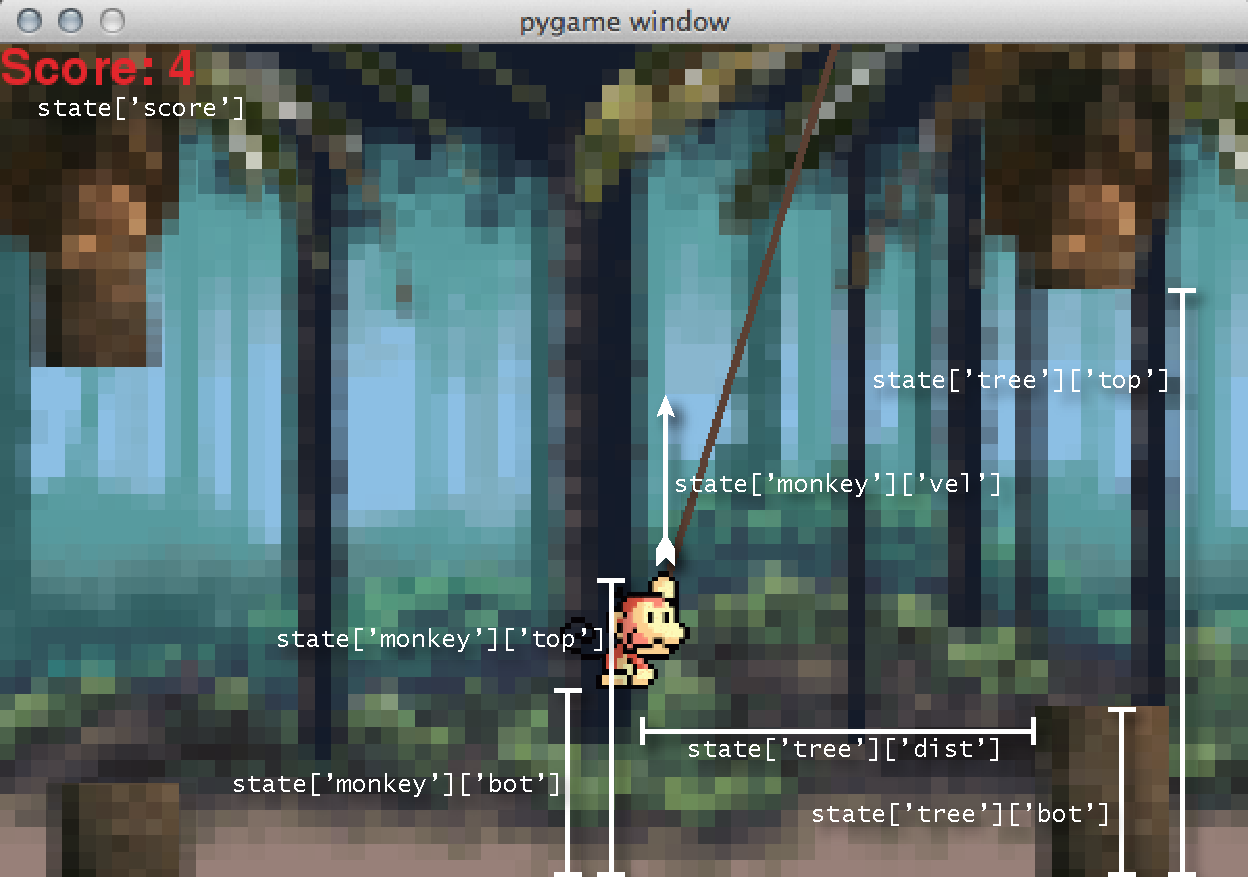
\includegraphics[width=0.48\textwidth]{figures/swingy-ann}
        \label{fig:swingy-ann}
    }
    \caption{(a) Screenshot of the Swingy Monkey game.  (b) Interpretations of various pieces of the state dictionary.}
\end{figure}
    
\textbf{Solution:}\\
I implemented Q-learning with an $\epsilon$-greedy policy in \texttt{stub.py} and then sought to improve performance by inferring gravity at each epoch in \texttt{stub\_grav.py}. The results were not as straightforward as may have been expected - inferring gravity did not improve results on all of the test metrics I discuss below.

\textit{\textbf{Implementation}}: In order to begin the Q-learning algorithm, we must have a tuple of the first (state, action, reward). By default, the monkey was initialized to not jump (action 0) from its starting state. Then, beginning with the second state, the monkey followed an $\epsilon$-greedy policy, taking a random next action with probability $\epsilon$ (exploring) and taking a greedy next action with probability $1 - \epsilon$ (exploiting, by taking the next action that maximized the Q-function). Regardless of this choice, the Q-function would be updated according to the update equation:
$$Q(s,a) \leftarrow Q(s,a) + \alpha[R(s,a) + \gamma \max_{a'} Q(s',a') - Q(s,a)] $$
where $Q(s,a)$ is the current value of the Q-function at state $s$ and taking action $a$ - $Q(s,a)$ starts by being initialized to 0 $\forall\, (s,a)$; $\alpha$ is the learning rate; $R(s,a)$ is the reward at state $s$ and taking action $a$; $\gamma$ is the discount rate on the value of future states and actions.

The only key difference between \texttt{stub.py} and \texttt{stub\_grav.py}, is that, in the former, $s$ is a tuple of $(x,y)$ - the discretized coordinates of the monkey - whilst, in the latter, $s$ is a tuple of $(x,y,g)$ - the discretized coordinates of the monkey and the level of gravity $g$ in the game. $g$ was calculated by finding the difference in the actual (not discretized) y-coordinate of the monkey between the first two states. In turned out that there were only two possible levels of gravity in the game, which I will refer to as ``low gravity" and ``high gravity". Intuitively, the monkey fell further between state 0 and state 1 in ``high gravity" games.

The theory behind inferring gravity was that the monkey would have a larger Q-table, from which it could learn about the different value of states and actions in low gravity and high gravity games, and thereby better optimize its policy.

\textit{\textbf{Results}}:
Using both \texttt{stub.py} and \texttt{stub\_grav.py}, I ran the game once (100 epochs) for several different values of the hyperparameters $\alpha$, $\gamma$, and $\epsilon$. I discovered that the values $\epsilon = 0.0001$, $\alpha = 0.1$, and $\gamma = 0.9$ produced the best scores.

In order to test the difference between \texttt{stub.py} and \texttt{stub\_grav.py} using the optimal parameters, I ran the game 50 times (100 epochs each time), and calculated the following metrics to demonstrate performance:
\begin{center}
    \begin{tabular}{ |c|c|c| } 
        \hline
        50 iterations & \texttt{stub.py} & \texttt{stub\_grav.py} \\
        \hline
        Average score across all epochs in all iterations & \mathcolorbox{green}{48.60} & 37.37\\
        \hline
        Max score across all epochs in all iterations & \mathcolorbox{green}{1416} & 1366\\
        \hline
        Average of max score in each iteration & \mathcolorbox{green}{753.28} & 652.98\\
        \hline
        Variance of max score in each iteration & 86258.12 & \mathcolorbox{green}{82978.98}\\
        \hline
    \end{tabular}
\end{center}

\newpage
\newpage
%%%%%%%%%%%%%%%%%%%%%%%%%%%%%%%%%%%%%%%%%%%%%
% Name and Calibration
%%%%%%%%%%%%%%%%%%%%%%%%%%%%%%%%%%%%%%%%%%%%%
\newpage
\subsection*{Name}
Ben Ray

\subsection*{Collaborators and Resources}
Whom did you work with, and did you use any resources beyond cs181-textbook and your notes?\\
Ty Geri\\
CS 181 OHs\\

\subsection*{Calibration}
Approximately how long did this homework take you to complete (in hours)?
14

\end{document}